\section{Controlled local inference comparison}
\label{sec:local-hardware}

This experiment measures the computational cost of the frozen PHASE-TTC system and the released Garl-TTC models on the same workstation. It uses real sensor inputs and does not read TTC labels, retrain weights, or submit predictions to a benchmark. Its purpose is to separate model capacity, runtime implementation, and input preparation. It does not establish a new accuracy ranking.

\subsection{Models and measurement protocol}

The PHASE arm loads the original nine-component distribution: four modality-specific motion producers, two pair heads, two temporal context refiners, and the residual fusion head. The complete system contains \LocalPhaseParameters{} parameters; the 1,955-parameter fusion head is only one component. Garl-TTC loads the published full, event-only, and RGB-only checkpoints with strict state-dictionary matching against frozen source and checkpoint hashes. The full model uses separate RGB and event ResNet-50 backbones, late feature fusion, and a height-ratio readout.

The released full Garl inference method also executes the auxiliary foreground decoders in both backbones. We therefore retain the unmodified release and add a separate decoder-bypass control using the same loaded weights with the native decoder flags disabled. Every query must preserve prepared input bytes, output availability, raw heights, and TTC, within $10^{-5}$ absolute and relative tolerance for numerical outputs. Bypass does not delete stored weights or produce a smaller exported checkpoint.

All arms run sequentially on the same NVIDIA GeForce RTX 5070 Ti Laptop GPU, with Python 3.11.15, PyTorch 2.11.0+cu128, CUDA 12.8, FP32, two PyTorch CPU threads, and TF32 disabled. The machine runs Windows with a shared desktop GPU. We preserve thermal, power, clock, and memory telemetry, and retain latency outliers. No second GPU experiment runs concurrently. These measurements describe this workstation and execution path; desktop scheduling and uncontrolled operating-system file caches remain sources of variation.

The main cohort contains all 434 supplied EvTTC query identities from ten recordings. Each of five arms processes every query in three passes, giving \LocalEvTTCAttempts{} measured attempts. Arm order rotates with query and pass. Each arm receives ten warmup calls at its first supported input; these are excluded and logged. Native representations and causal histories differ between models. PHASE uses up to 650\,ms of history, whereas Garl uses its corresponding current pair. Both use supplied object regions; detection and sensor acquisition are outside the measured boundary.

Preparation time includes native sensor access, decoding, region transforms, and representation construction. Prepared inference starts with host arrays and ends with the host TTC result, including transfer, synchronization, and runtime API diagnostics. Total time is the sum of these two intervals. Loading, reader initialization, hashing, logging, and warmup are excluded. Cyclic rotation does not balance all ordered arm pairs; order, thermal state, and scheduling limit causal interpretation of latency differences. The EvTTC arms also share a sensor reader, so shared cache state specifically affects preparation comparisons. The portable PHASE EvTTC API reconstructs the query history; it is distinct from the persistent paced service in Section~\ref{sec:runtime}. We do not infer a speed ratio between those separate implementations.

\subsection{Capacity, memory, and observed arithmetic}

\begin{table}[H]
\centering\small
\caption{\textbf{Complete original PHASE parameter inventory.} Counts come from the strictly loaded distributed components. All nine components contribute to the full \LocalPhaseParameters{}-parameter total.}
\begin{tabular}{lrr}
\toprule
Component & Parameters & Share \\
\midrule
Event transport producer & 424,274 & 18.07\% \\
Event coarse-to-fine producer & 424,293 & 18.08\% \\
RGB transport producer & 417,074 & 17.77\% \\
RGB coarse-to-fine producer & 417,093 & 17.77\% \\
Event pair head & 17,547 & 0.75\% \\
RGB pair head & 17,547 & 0.75\% \\
Event temporal refiner & 313,765 & 13.37\% \\
RGB temporal refiner & 313,765 & 13.37\% \\
Residual phase fusion head & 1,955 & 0.08\% \\
\bottomrule
\end{tabular}

\end{table}

\begin{table}[H]
\centering\small
\caption{\textbf{Capacity and separately profiled computation.} Stored counts include every unique parameter in the loaded graph. Executed counts include parameters owned by modules called on one real, supported full-history query. Peak memory is PyTorch CUDA allocated memory with only the profiled arm resident; the bypass retains decoder weights. Counted arithmetic covers profiler-supported operators and is not a complete FLOP count.}
\label{tab:local-capacity}
\begin{tabular}{lrrrr}
\toprule
Model & Stored M & Executed M & Peak MiB & Counted GFLOPs \\
\midrule
PHASE-TTC & 2.347 & 2.347 & 41.2 & 29.22 \\
Garl full release & 243.110 & 243.110 & 1416.6 & 54.69 \\
Garl decoder bypass & 243.110 & 49.240 & 984.9 & 6.37 \\
Garl event-only & 24.674 & 24.674 & 147.9 & 3.62 \\
Garl RGB-only & 24.568 & 24.568 & 144.9 & 2.75 \\
\bottomrule
\end{tabular}

\end{table}

On the profiled query, PHASE executes modules owning \LocalPhaseExecutedParameters{} parameters, compared with \LocalGarlTTCParameters{} for decoder-bypassed Garl: \LocalExecutedParameterReduction{} fewer observed executed parameters. These counts describe the measured paths and do not establish a minimal exported Garl model. The bypass control retains the complete published checkpoint in memory. Comparisons of stored capacity include Garl's auxiliary decoder branches, as shown in Table~\ref{tab:local-capacity}.

Hooks and the operator profiler run separately from latency trials. Memory profiling moves the other model weights to the CPU before measuring allocated and reserved CUDA peaks. Process RSS includes the Python process and host allocations, so it is retained in the evidence rather than presented as model-only memory. Supported-operator FLOPs omit or incompletely represent recurrent and custom transport operations; they do not measure full algorithmic complexity or predict wall-clock latency.

\subsection{EvTTC inference and sensor preparation}

\begin{table}[H]
\centering\small
\caption{\textbf{EvTTC prepared-input-to-host inference, in milliseconds.} Timing uses the \LocalMatchedQueries{} unique queries successful in all five arms, repeated three times. Coverage retains all planned attempts, including unavailable predictions.}
\label{tab:local-inference}
\begin{tabular}{lrrrrr}
\toprule
Model & Outputs/attempts & Mean & Median & p95 & p99 \\
\midrule
PHASE-TTC & 1302/1302 & 501.48 & 530.26 & 651.37 & 668.75 \\
Garl full release & 1272/1302 & 60.00 & 36.94 & 219.92 & 273.93 \\
Garl decoder bypass & 1272/1302 & 13.09 & 10.40 & 33.15 & 41.12 \\
Garl event-only & 1302/1302 & 6.76 & 5.42 & 19.15 & 35.83 \\
Garl RGB-only & 1278/1302 & 7.34 & 5.24 & 17.91 & 31.56 \\
\bottomrule
\end{tabular}

\end{table}

\begin{table}[H]
\centering\small
\caption{\textbf{EvTTC preparation and total cost, in milliseconds.} The same all-five complete-case population is used. Total includes preparation and synchronized native inference.}
\label{tab:local-pipeline}
\begin{tabular}{lrrrr}
\toprule
Model & Prep. mean & Total mean & Total median & Total p95 \\
\midrule
PHASE-TTC & 847.07 & 1348.55 & 1369.64 & 2508.53 \\
Garl full release & 370.53 & 430.54 & 416.53 & 824.82 \\
Garl decoder bypass & 369.95 & 383.04 & 378.58 & 721.76 \\
Garl event-only & 258.35 & 265.12 & 251.91 & 598.11 \\
Garl RGB-only & 113.13 & 120.47 & 126.85 & 137.10 \\
\bottomrule
\end{tabular}

\end{table}

On these matched queries, median prepared inference is \LocalEvPhaseInferMedian{}\,ms for PHASE, \LocalEvGarlFullInferMedian{}\,ms for full Garl, and \LocalEvGarlBypassInferMedian{}\,ms for decoder-bypassed Garl. Median total cost is respectively \LocalEvPhaseTotalMedian{}, \LocalEvGarlFullTotalMedian{}, and \LocalEvGarlBypassTotalMedian{}\,ms. Model size and latency must therefore be reported separately: the parameter reduction alone does not support a claim of faster inference.

\subsection{Native RAW replay on eAP}

The second cohort selects the first ten chronological physical queries in each of the twelve frozen eAP Test12 sequences, after collapsing aliases: 120 queries and \LocalEAPAttempts{} measured attempts across three arms and three passes. Selection uses identities and timestamps, without prediction or label filtering. It is a deterministic prefix cohort, not a random sample of the entire benchmark.

PHASE uses its native causal predictor with per-sequence observation reuse. Its event tensors are reconstructed from real HDF5 events and required to match the frozen input tensors exactly before timing. Garl receives the corresponding supplied current RGB/event pair through its native normalization and 40-plane event representation. Both methods read real sensor data, but use separate per-sequence readers and their native caching behavior. Each arm receives three first-query warmup calls per sequence, after which readers and PHASE observation caches are reset; operating-system caches are not flushed. Each pass resets sequence state.

Garl's eAP TTC conversion preserves the released model's nominal $\Delta t=0.1$\,s. The observed sensor-clock pair intervals are recorded separately; their small clock-mapping differences do not change the native conversion rule. This differs from the explicitly measured-cadence adaptation used on EvTTC. Full and bypass outputs, inputs, and availability must agree for every selected query, and repeated outputs must remain within the same numerical tolerance.

\begin{table}[H]
\centering\small
\caption{\textbf{eAP native RAW-to-host cost, in milliseconds.} The clock includes real sensor reading, preparation, native computation, and host output. Timings use queries successful in all three arms; coverage includes all attempts. This replay includes PHASE observation reuse and is separate from the EvTTC portable API and the 50\,Hz paced-service experiment.}
\label{tab:local-eap}
\begin{tabular}{lrrrrr}
\toprule
Model & Outputs/attempts & Mean & Median & p95 & p99 \\
\midrule
PHASE native RAW & 360/360 & 362.56 & 342.45 & 615.19 & 756.00 \\
Garl full RAW & 360/360 & 235.45 & 224.02 & 368.19 & 578.85 \\
Garl bypass RAW & 360/360 & 204.52 & 202.31 & 323.26 & 364.97 \\
\bottomrule
\end{tabular}

\end{table}

Median native RAW-to-host cost is \LocalEAPPhaseTotalMedian{}\,ms for PHASE, \LocalEAPGarlFullTotalMedian{}\,ms for full Garl, and \LocalEAPGarlBypassTotalMedian{}\,ms for the bypass control. These results describe the stated prefix replay and native implementations. They do not establish camera-to-warning response, sustained multi-object operation, or an optimized deployment limit.

\subsection{Coverage, pairwise comparisons, and variation}

\begin{figure}[H]
\centering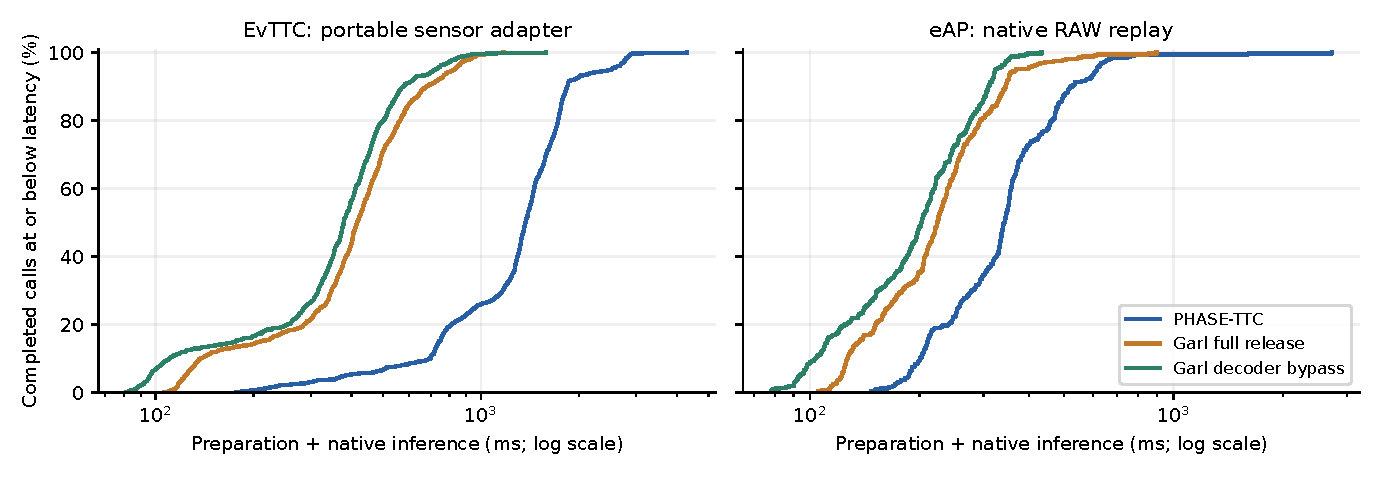
\includegraphics[width=\linewidth]{figures/local_latency_cdf.pdf}
\caption{\textbf{Complete measured latency distributions.} Each panel uses its all-model complete-case population over three passes. The horizontal axis is logarithmic. Input histories, cache reuse, and native runtime paths differ between cohorts; curves compare arms within each panel.}
\end{figure}

\begin{table}[H]
\centering\small
\caption{\textbf{All-attempt total cost, in milliseconds.} Unavailable predictions remain in the denominator and their processing time remains in these distributions. They are not treated as completed TTC estimates.}
\begin{tabular}{llrrrrr}
\toprule
Cohort & Model & Calls & Mean & Median & p95 & p99 \\
\midrule
EvTTC & PHASE-TTC & 1302 & 1319.64 & 1360.79 & 2445.55 & 2853.16 \\
EvTTC & Garl full release & 1302 & 420.93 & 412.65 & 824.00 & 960.37 \\
EvTTC & Garl decoder bypass & 1302 & 374.52 & 375.88 & 718.42 & 885.01 \\
EvTTC & Garl event-only & 1302 & 259.77 & 250.22 & 596.96 & 757.84 \\
EvTTC & Garl RGB-only & 1302 & 118.05 & 126.72 & 137.05 & 148.49 \\
eAP & PHASE native RAW & 360 & 362.56 & 342.45 & 615.19 & 756.00 \\
eAP & Garl full RAW & 360 & 235.45 & 224.02 & 368.19 & 578.85 \\
eAP & Garl bypass RAW & 360 & 204.52 & 202.31 & 323.26 & 364.97 \\
\bottomrule
\end{tabular}

\end{table}

\begin{table}[H]
\centering\small
\caption{\textbf{Pairwise complete-case total medians, in milliseconds.} Each row uses only the two named methods' jointly successful query/pass identities. Failure of an unrelated modality-only control does not remove a pairwise observation.}
\begin{tabular}{llrrr}
\toprule
Cohort & Comparator & Paired calls & PHASE median & Garl median \\
\midrule
EvTTC & Garl full release & 1272 & 1369.64 & 416.53 \\
EvTTC & Garl decoder bypass & 1272 & 1369.64 & 378.58 \\
EvTTC & Garl event-only & 1302 & 1360.79 & 250.22 \\
EvTTC & Garl RGB-only & 1278 & 1368.04 & 126.84 \\
eAP & Garl full RAW & 360 & 342.45 & 224.02 \\
eAP & Garl bypass RAW & 360 & 342.45 & 202.31 \\
\bottomrule
\end{tabular}

\end{table}

\begin{table}[H]
\centering\small
\caption{\textbf{Total means by repeated pass, in milliseconds.} The all-model complete-case population is retained within each cohort. These are repeated timing passes with frozen weights, not independent training seeds.}
\begin{tabular}{llrrr}
\toprule
Cohort & Model & Pass 1 & Pass 2 & Pass 3 \\
\midrule
EvTTC & PHASE-TTC & 1339.11 & 1361.48 & 1345.05 \\
EvTTC & Garl full release & 421.70 & 426.35 & 443.55 \\
EvTTC & Garl decoder bypass & 381.66 & 386.24 & 381.23 \\
eAP & PHASE native RAW & 369.67 & 352.58 & 365.43 \\
eAP & Garl full RAW & 242.58 & 232.21 & 231.56 \\
eAP & Garl bypass RAW & 206.29 & 201.59 & 205.67 \\
\bottomrule
\end{tabular}

\end{table}

\begin{table}[H]
\centering\small
\caption{\textbf{Total medians by recording, in milliseconds.} Counts are unique queries in the all-model complete-case population; each has three measured passes.}
\begin{tabular}{llrrrr}
\toprule
Cohort & Recording & Queries & PHASE & Garl full & Garl bypass \\
\midrule
EvTTC & CCRm-low & 41 & 1703.29 & 487.29 & 455.53 \\
EvTTC & CCRm-medium & 39 & 1559.72 & 546.41 & 433.32 \\
EvTTC & CCRs1-high & 29 & 2691.82 & 841.28 & 764.00 \\
EvTTC & CCRs1-low & 49 & 1268.63 & 405.70 & 357.42 \\
EvTTC & CCRs1-medium & 42 & 1304.52 & 407.48 & 349.94 \\
EvTTC & CCRs2-high & 58 & 1653.90 & 476.86 & 453.12 \\
EvTTC & CCRs2-low & 45 & 1274.72 & 367.93 & 340.55 \\
EvTTC & CCRs2-medium & 54 & 1487.52 & 427.14 & 398.60 \\
EvTTC & Slider-1000 & 18 & 788.75 & 142.98 & 113.61 \\
EvTTC & Slider-750 & 49 & 727.47 & 125.96 & 97.65 \\
eAP & 3RUZHwnCwK & 10 & 306.32 & 208.96 & 181.68 \\
eAP & 71wUSQYMpk & 10 & 254.30 & 160.98 & 143.59 \\
eAP & 89fvtHGHx2 & 10 & 360.36 & 254.20 & 233.71 \\
eAP & HHJe79eY2J & 10 & 495.18 & 300.78 & 278.02 \\
eAP & JcjcDPISuL & 10 & 364.32 & 242.24 & 215.38 \\
eAP & M8I2irMvY7 & 10 & 190.49 & 126.16 & 98.97 \\
eAP & Mu6kaUjIz3 & 10 & 616.10 & 354.50 & 326.47 \\
eAP & V741M41vPW & 10 & 356.01 & 224.56 & 212.78 \\
eAP & kafYzX6kJ4 & 10 & 204.50 & 127.24 & 109.01 \\
eAP & nP4MRdpEeO & 10 & 338.60 & 221.35 & 198.07 \\
eAP & r0PXQOpCA6 & 10 & 211.56 & 137.52 & 111.19 \\
eAP & vhjB5OViA7 & 10 & 455.30 & 315.82 & 295.03 \\
\bottomrule
\end{tabular}

\end{table}

The evidence directory \texttt{data/local\_hardware\_20261112/} contains the pre-run protocols, complete trial ledgers, telemetry, loading bindings, parity evidence, and separate profiles. Source and checkpoint hashes identify the executed code and weights. The table generator rejects partial populations, duplicate attempts, changed protocol or trial hashes, nonfinite timings, and failed parity checks. Every table is regenerated from these records; no measured value is entered manually into the manuscript.
